\documentclass{beamer}
\usetheme{Singapore}
\setbeamercovered{transparent}

\usepackage[english]{babel}
\usepackage[utf8]{inputenc}
\usepackage{times}
\usepackage[T1]{fontenc}
\usepackage{graphicx}
\usepackage{ragged2e}
\justifying

\title{Exploratory Data Analysis\\On Genetic Data}
\date{\small MATH 252 Final Presentation \newline Supervisor: Mr. Kiran Shrestha\newline
Special Thanks to Mr. Simon Shrestha}
\institute{Kathmandu University \\ Department of Computational Mathematics}
\author{Aayush Shrestha \and Anmol Jha}

\subject{Exploratory Data Analysis}
\begin{document}
	
	\justifying
	\begin{frame}
		\titlepage
	\end{frame}
	\pagenumbering{}
	\begin{frame}{Outline}
		\begin{enumerate}
			\item Introduction
			\item Methodology
			\item Completed Work
			\item Conclusion
		\end{enumerate}
	\end{frame}
	
	\section{Introduction}
	\begin{frame}{Exploratory Data Analysis}
		Exploratory Data Analysis (EDA) is a method of analyzing data using statistical summaries and graphical representations.\newline \newline
		
		EDA is a critical process that aids in determining how to best manipulate data sources to obtain the required answers, making it easier for data scientists to discover patterns, detect anomalies, determine test hypotheses, and validate assumptions.
	\end{frame}
	
	\begin{frame}{Dashboard}
		A dashboard is basically a GUI for Data Visualization. A dashboard is a good choice if you need to summarize and present a lot of information on a single window.\newline \newline
		
		A dashboard helps Data Analysts and Data Scientists perform many data-related tasks and also provides a visual aid for other stakeholders to understand data and make accurate data-based decisions.
	\end{frame}
	\begin{frame}{Project}
		Our project consist of the task to perform EDA on a Kaggle dataset so as to find the significant attributes that contribute to the classification of the target genetic disorder.\\
		Also we were to create a dashboard including all those Key performance indicators. 
	\end{frame}	
	\begin{frame}{Initial View}
		\begin{figure}
			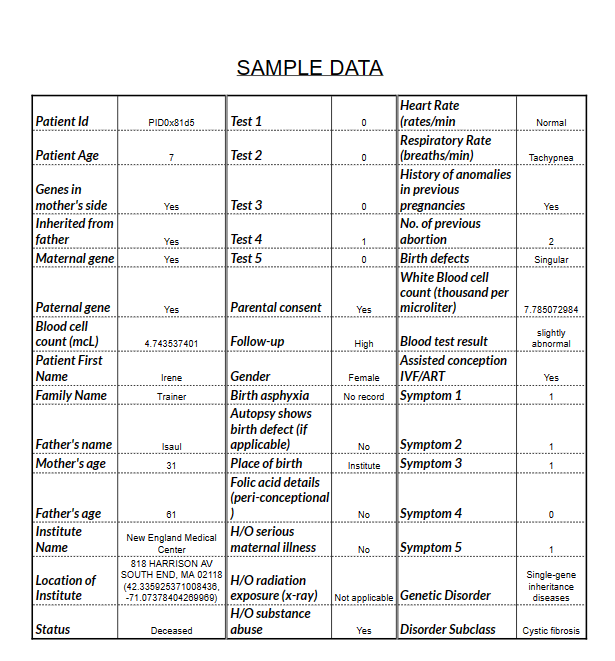
\includegraphics[width=0.65\textwidth, height=0.72\textheight]{sample.png}
			\caption{Sample raw data.}
		\end{figure}
	\end{frame}
	\section{Methodology}
	\begin{frame}{Non Graphical}
		Initially we used the summary statistics, count, minimum, maximum, average, standard deviation etc to describe the numeric columns. \\
		Also correlation between every pair of numeric attributes were computed to find highly correlated attributes.\\ 
	\end{frame}
	\begin{frame}{Graphical}
		We used R programming packages to create visualization related to the distribution of an attribute on its own and also to demonstrate the relation between attributes. Here we mainly used ggplot package to create stacked bar graph and stem and leaf plots.\\
		Also we used a heat-map plot to better visualize the correlation matrix created.
	\end{frame}
	\begin{frame}{Domain Based}
	Based on the further continuation of the project as a classification of genetic disorder based on genetic inheritance the attributes were considered for their significane to the project and promptly discarded.
	\end{frame}
	\begin{frame}{Dashboard}
		We used \url{https://visual.is} as a proper dashboard creation tool. This let us interactively choose different plots and data that we want to display in our dashboard.
	\end{frame}
	\section{Completed Work}
	\begin{frame}{Initial Pre-processing}
		The data was changed from an \underline{xlsx} file to a \underline{csv} file, and the column names were modified to better suit programming. Also, all the rows with any NA values were removed.The dataset now contains 45 columns and 6706 observations.
			\begin{figure}
				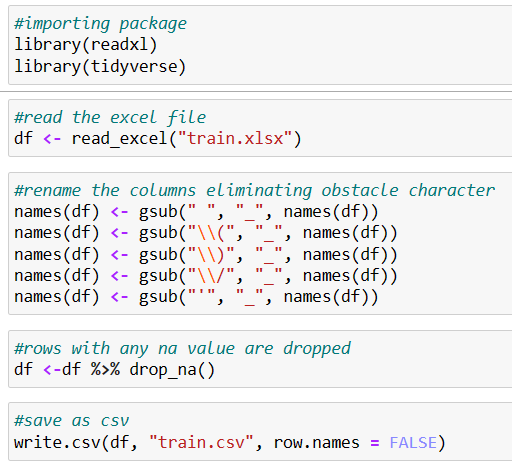
\includegraphics[width=0.65\textwidth, height=0.6\textheight]{pre.png}
				\caption{Preprocessing Code.}
			\end{figure}
		
	\end{frame}
	
	\begin{frame}{Non Graphical EDA}
		Summary statistics showed that the columns of Test 1, Test 2,, Test 3, Test 4, Test 5 have no variance in them hence they are removed.
		\begin{figure}
			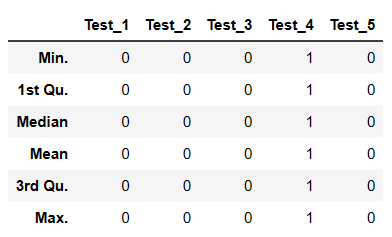
\includegraphics[width=0.65\textwidth, height=0.6\textheight]{s_stat.png}
			\caption{Summary Statistics}
		\end{figure}
	\end{frame}
	\begin{frame}{Non Graphical EDA}
		Also a correlation heatmap showed that there are no highly correlated attribute
		\begin{figure}
			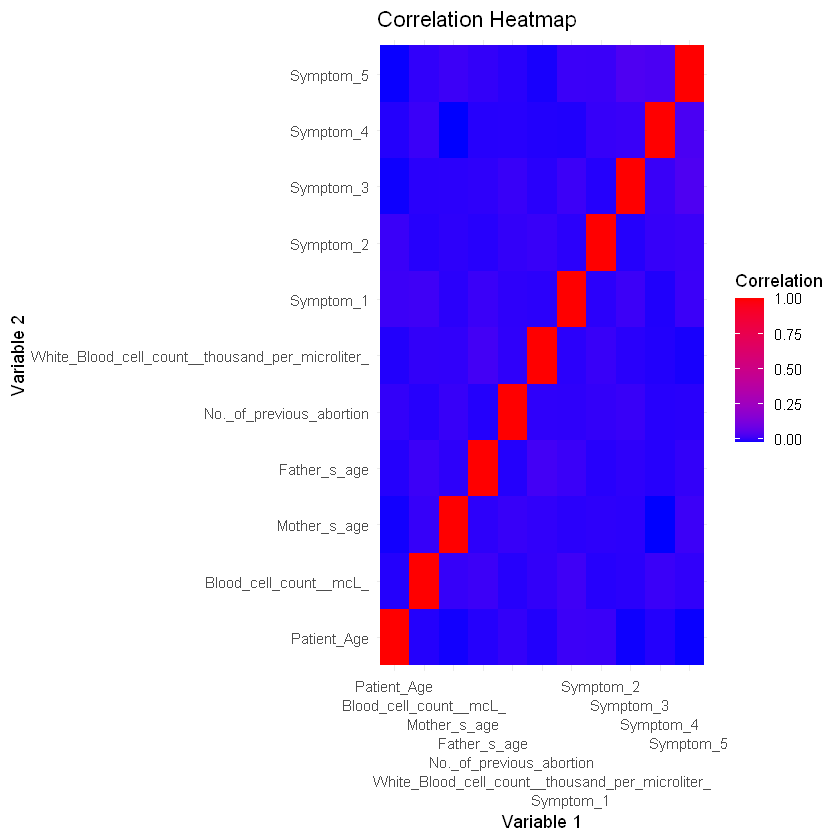
\includegraphics[width=0.65\textwidth, height=0.6\textheight]{corr.png}
			\caption{Correlation Heatmap}
		\end{figure}
	\end{frame}
		\begin{frame}{Graphical EDA}
		We find that the Genetic disorder attribute is dependent on the Disorder Subclass attribute. Hence The Genetic Disorder attribute is removed.
		\begin{figure}
			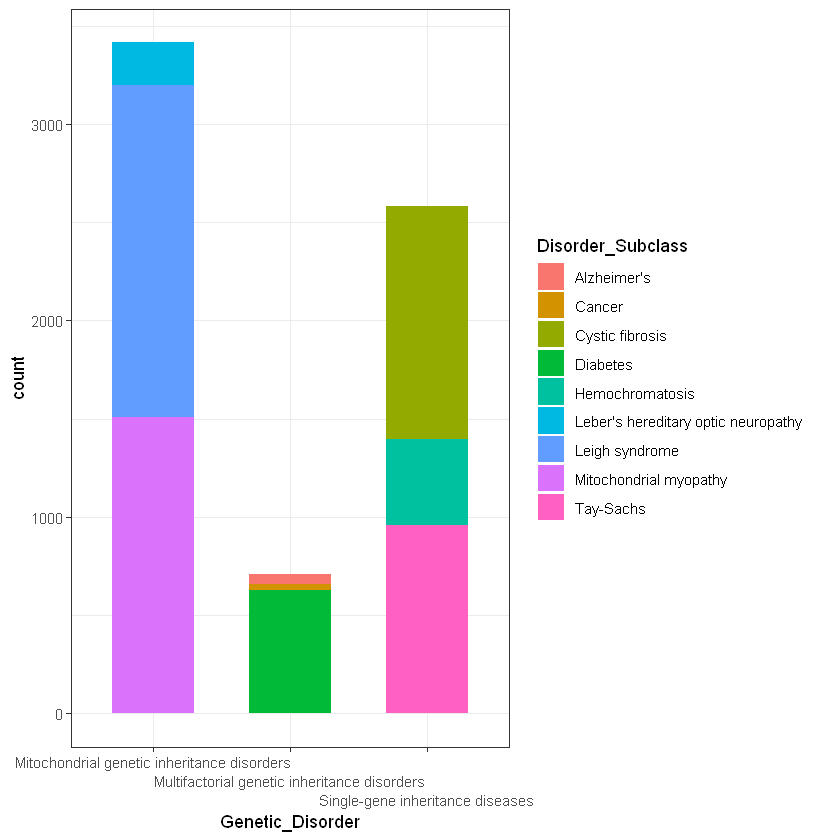
\includegraphics[width=0.65\textwidth, height=0.6\textheight]{rel.png}
			\caption{Dependency between Target Attributes}
		\end{figure}
	\end{frame}
\begin{frame}{Graphical EDA}
For categorical attributes, a stacked bar graph is created with Disorder subclass attribute on x-axis. By this we found that most of such attributes divided the dataset almost symmetrically along the Disorder Subclass and hence is removed.

\begin{figure}
	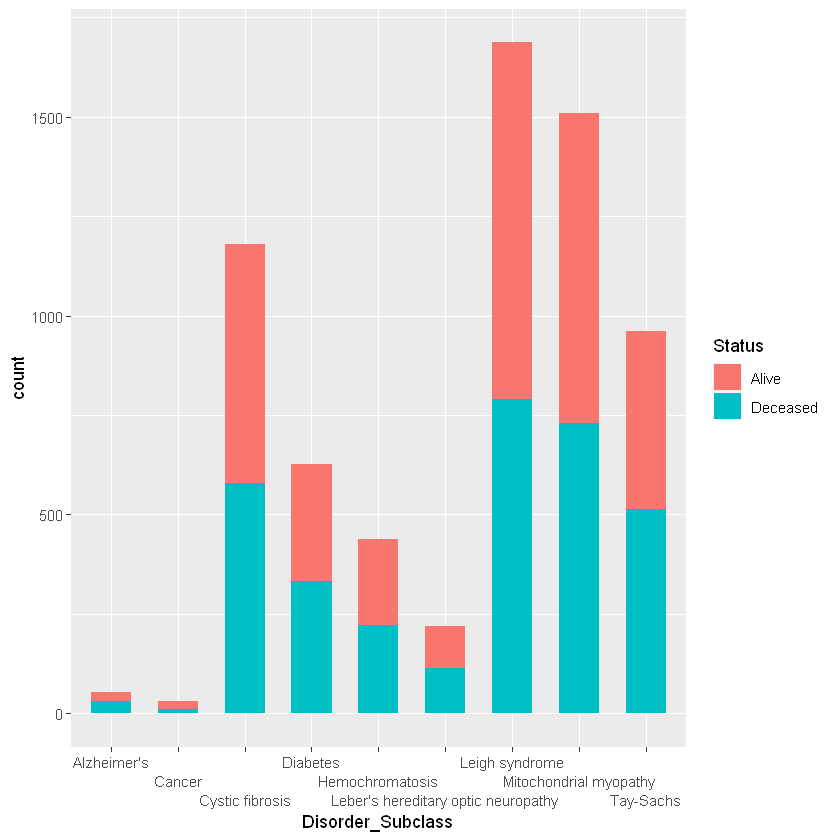
\includegraphics[width=0.65\textwidth, height=0.6\textheight]{status.png}
	\caption{Disorder Subclass and Status}
\end{figure}
\end{frame}

\begin{frame}{Graphical EDA}
	For continuous attributes, a box and whisker plot is created with Disorder subclass attribute on x-axis. Here the data were not as symmetrical.
	
	\begin{figure}
		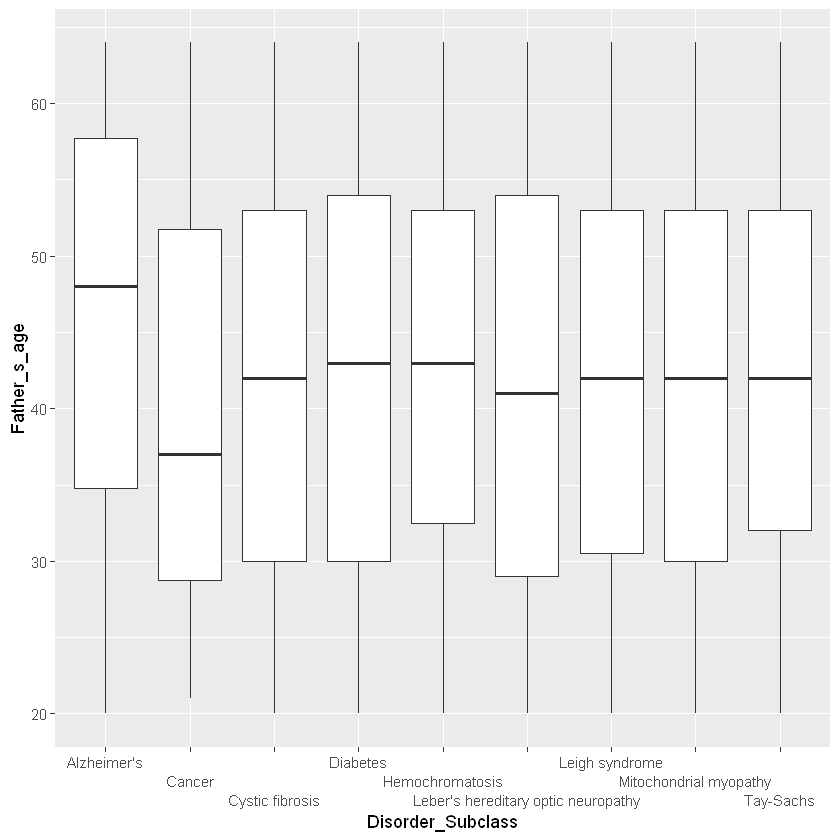
\includegraphics[width=0.65\textwidth, height=0.6\textheight]{f-age.png}
		\caption{Disorder Subclass and Patient's Father's age}
	\end{figure}
\end{frame}

\begin{frame}{Graphical EDA + Domain Information}
	Given the domain of study to be classification of disorder due to genetic inheritance, the following attribute were considered significant and have shown reliable variance.
	
	\begin{figure}
		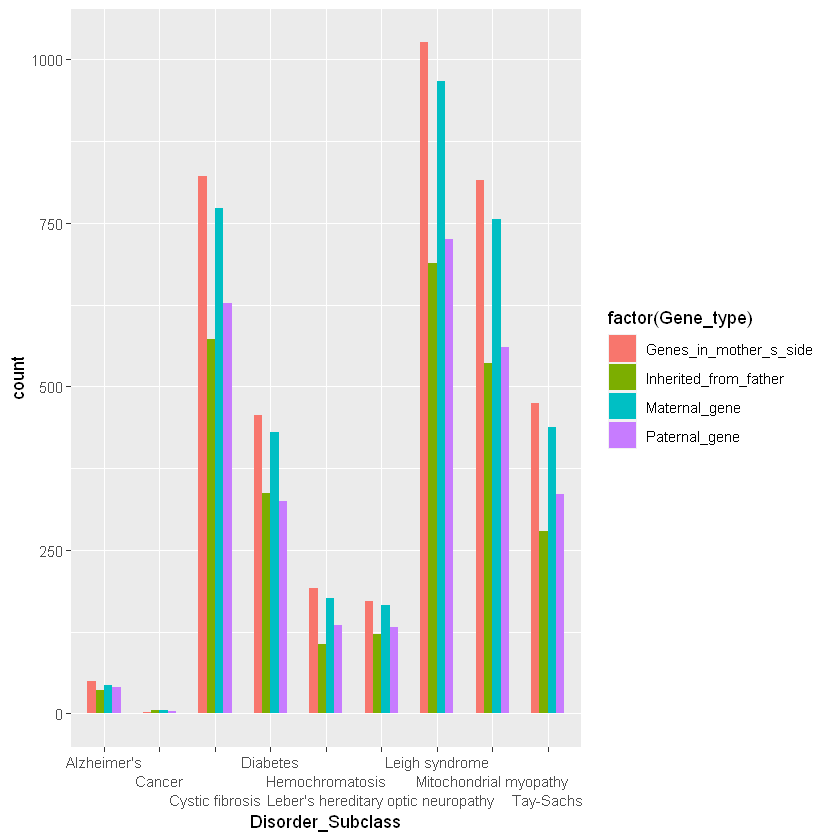
\includegraphics[width=0.65\textwidth, height=0.6\textheight]{gy.png}
		\caption{Disorder Subclass and Genetic Presence (YES)}
	\end{figure}
\end{frame}

\begin{frame}{Graphical EDA + Domain Information}
	
	\begin{figure}
		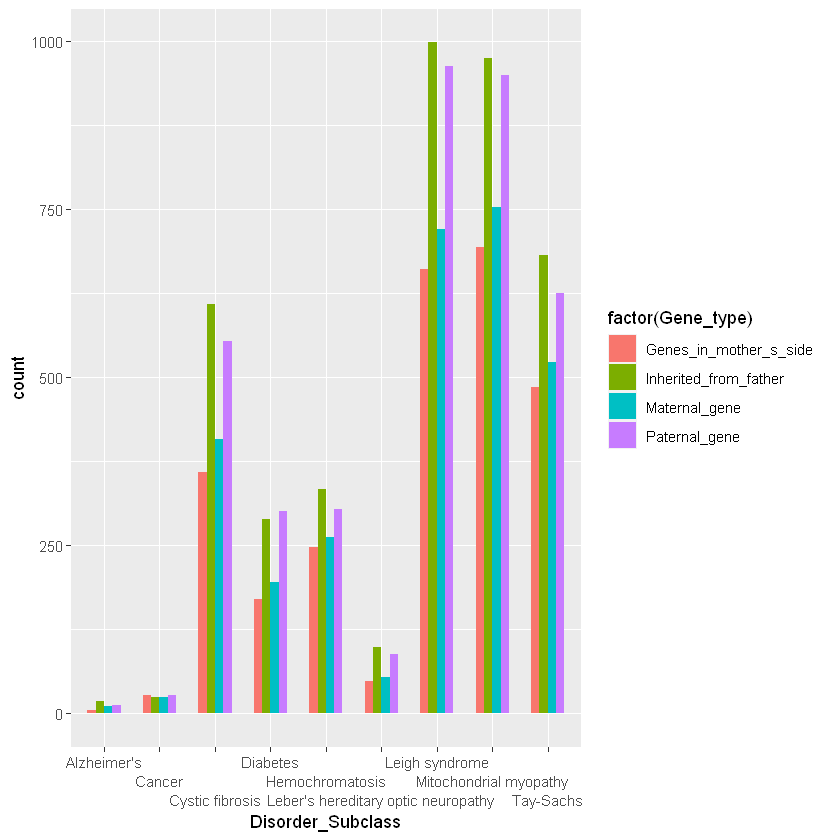
\includegraphics[width=0.65\textwidth, height=0.6\textheight]{gn.png}
		\caption{Disorder Subclass and Genetic Presence (NO)}
	\end{figure}
\end{frame}

\begin{frame}{Graphical EDA + Domain Information}

	\begin{figure}
		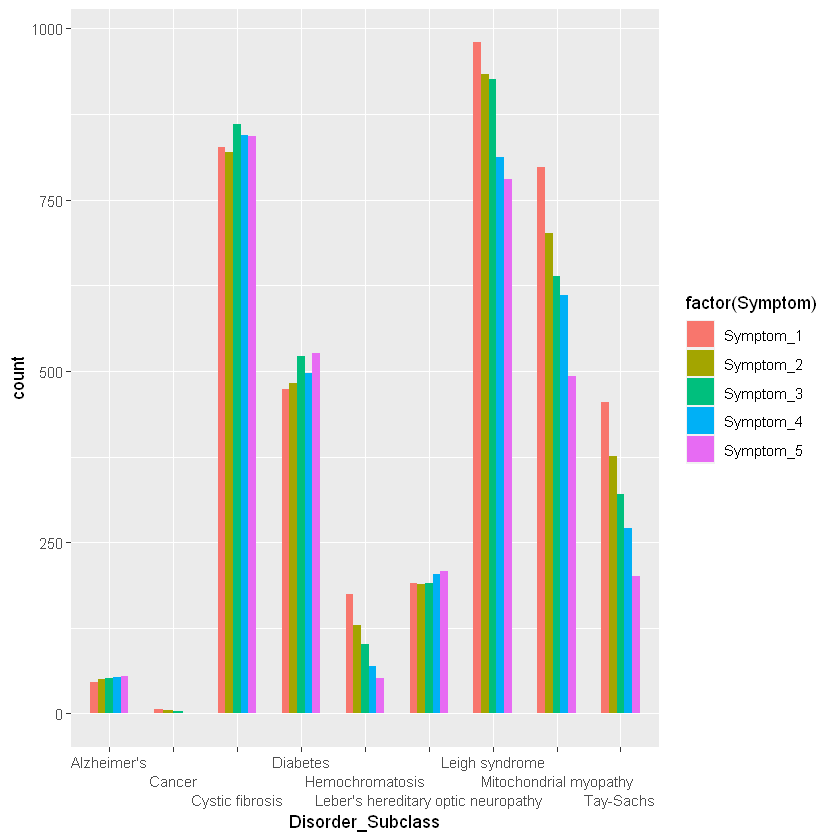
\includegraphics[width=0.65\textwidth, height=0.6\textheight]{s1.png}
		\caption{Disorder Subclass and Symptom Detected (True)}
	\end{figure}
\end{frame}

\begin{frame}{Graphical EDA + Domain Information}
	
	\begin{figure}
		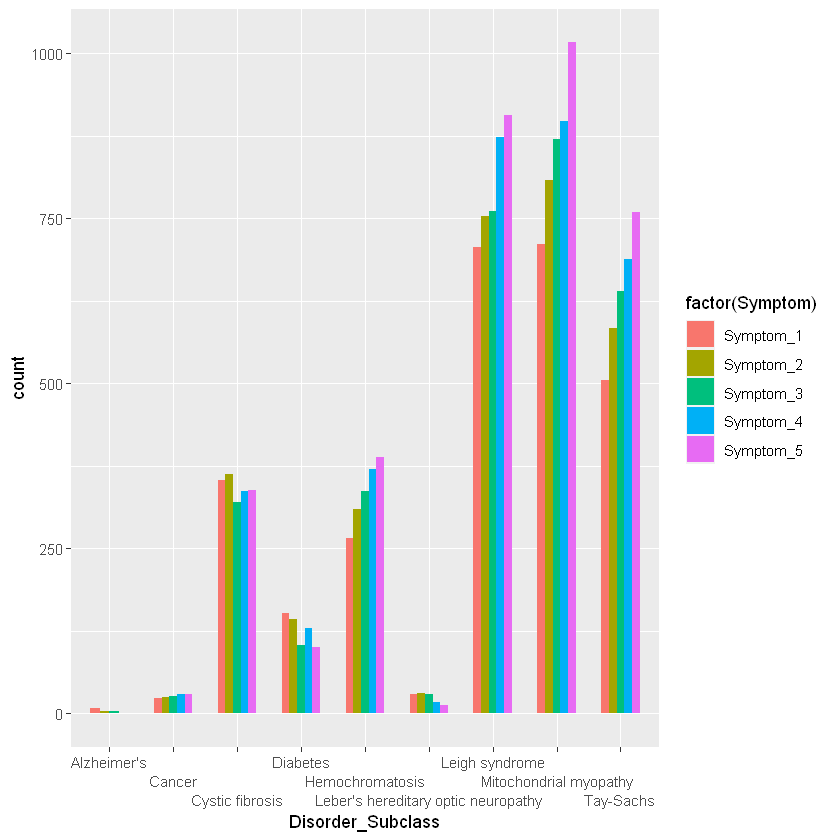
\includegraphics[width=0.65\textwidth, height=0.6\textheight]{s0.png}
		\caption{Disorder Subclass and Symptom Detected (False)}
	\end{figure}
\end{frame}
\begin{frame}{Domain Based}
	Attributes like Patients Name, birth address, History of alcohol which doesnt have much significance to the domain of genetic inheritance were also removed.\\
	All this left us with 16 columns with one of them being the target column.
\end{frame}
	\begin{frame}{Dashboard}
		We have a basic dashboard framework ready that  gives us basic visualization of the data.
			\begin{figure}
			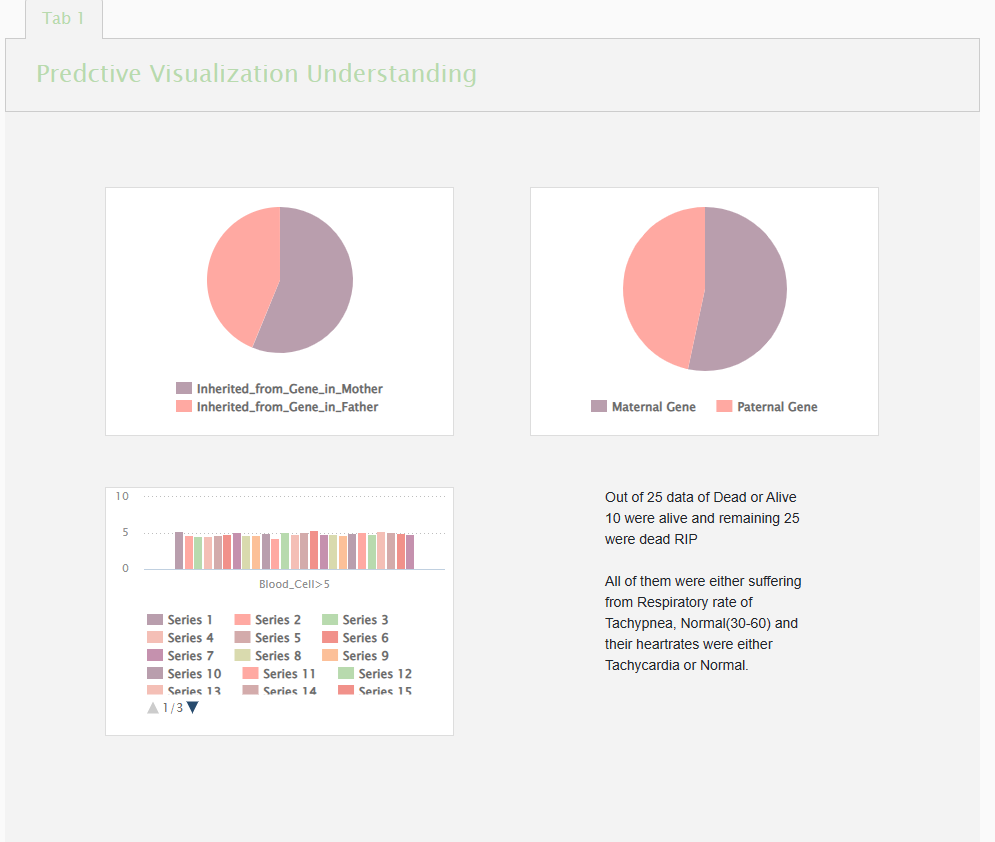
\includegraphics[width=0.65\textwidth, height=0.6\textheight]{dash.png}
			\caption{Dashboard Sample}
		\end{figure}
	\end{frame}
	
	\section{Conclusion}
	\begin{frame}{Conclusion}
		In this EDA project, we applied various statistical analysis, graphical visualization, and domain knowledge to reduced the dataset from 45 to 16 columns.
		\begin{table}[htpb]
			\centering
			\begin{tabular}{|l|l|}
				\hline
				Patient Age&				Genes in mother's side\\
				Inherited from father &				Maternal gene\\
				Paternal gene &				Blood cell count mcL\\
				Mother's age &				Father's age\\
				Number of previous abortion &				White Blood cell count \\
				Symptom 1 &				Symptom 2\\
				Symptom 3&				Symptom 4\\
				Symptom 5 &                     	Disorder Subclass\\ 
				\hline
			\end{tabular}
			\label{tab 2}
		\end{table}
	\end{frame}
	\begin{frame}{Discussion and Limitations}
	The dashboard created is entirely dependent on the capability of the tool used.\\ 
	Given that the data is from a Kaggle dataset, there is a possibility of it being synthetic, as such there are certain trends and outliers that isnt explainable from a real world perspective.\\
	
	The methodology discussed here is still useful and backed by proper citable sources. Hence there are still proper real world application of this project and or its workflow. 

	\end{frame}	

	\begin{frame}{Demonstration}
	\begin{center}
		{\Huge Now we  would like to demonstrate the Project} \newline \newline
		
		
	\end{center}
	
\end{frame}	

	\section*{}
	\begin{frame}
		\begin{center}
			{\Huge THANK YOU!} \newline \newline
		Please share if you have any queries.\newline \newline
		We would like to show the code now.
		
	\end{center}
	\end{frame}
	
\end{document}
